\chapter{Additional Code Examples} \label{App:AppendixA}
\section{Statistics}
\subsection{Polynomial Fit}
\begin{figure}[h!]
	\centering
	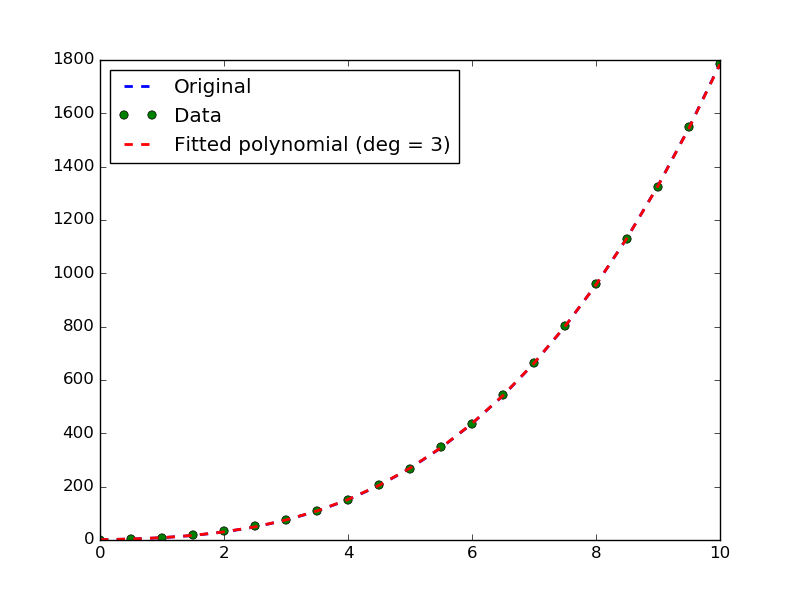
\includegraphics[width=\linewidth]{images/poly_fit.png}
    \caption{Polynomial fit to noisy data}
\end{figure}
\newpage
\noindent\begin{minipage}{\linewidth}
\begin{lstlisting}[style=python]
import pandas as pd
import numpy as np
import matplotlib.pyplot as plt
import scipy.optimize as spo

def error_poly(C,data):
	return np.sum((data[:,1] - np.polyval(C,data[:,0])) ** 2)

def fit_poly(data,error_func,degree=3):
	guess = np.poly1d(np.ones(degree+1, dtype=np.float32))

	return spo.minimize(error_func, guess, args=(data,), method='SLSQP', options={'disp':True}).x

def test_run():
	original_poly = np.float32([1.5,2.5,3.5,1])

	Xoriginal = np.linspace(0,10,21)
	Yoriginal = np.polyval(original_poly,Xoriginal)
	plt.plot(Xoriginal,Yoriginal,'b--',linewidth=2.0,label="Original")

	noise_sigma = 2
	noise = np.random.normal(0,noise_sigma,Yoriginal.shape)

	data = np.asarray([Xoriginal,Yoriginal+noise]).T

	degree = 3
	poly = fit_poly(data,error_poly,degree)

	plt.plot(data[:,0],data[:,1],'go',label="Data")

	plt.plot(data[:,0],np.polyval(poly,data[:,0]),'r--',linewidth=2.0,label="Fitted polynomial (deg = {})".format(degree))
	plt.legend(loc='upper left')
	plt.show()

if __name__ == "__main__":
	test_run()
\end{lstlisting}
\end{minipage}

\section{Algorithms}
\subsection{kNN Learner}
\noindent\begin{minipage}{\linewidth}
\begin{lstlisting}[style=python]
import numpy as np

class KNNLearner(object):
	def __init__(self, k):
		self.k = k
		self.x = None
		self.y = None

	def addEvidence(self, X,Y):
		if(self.x is None):
			self.x = X
			self.y = Y
		else:
			self.x = np.vstack((self.x, X))
			self.y = np.append(self.y, Y)

	def query(self, points):
		ret = np.array([])
		for point in points:
			ret = np.append(ret, self.y[np.linalg.norm(self.x-point,axis=1).argsort()[:self.k]].mean())	# get the k closest x locations, then find the mean of their y values
		return ret
\end{lstlisting}
\end{minipage}

\noindent Running this on some 2-dimensional x testing data, we can compare the linear regression learner to the kNN learner:

\noindent\begin{minipage}{\linewidth}
\begin{lstlisting}[style=python]
==== kNNLearner =====
In sample results
RMSE:  0.293210201429
corr:  0.933616301402

Out of sample results
RMSE:  0.40276819912
corr:  0.867504170015

==== LinRegLearner =====
In sample results
RMSE:  0.515854106381
corr:  0.776302806055

Out of sample results
RMSE:  0.52366864612
corr:  0.758354066174
[Finished in 0.1s]
\end{lstlisting}
\end{minipage}
\noindent The kNN learner was run with $k = 3$.

\subsection{kNN Bag Learner}
\noindent\begin{minipage}{\linewidth}
\begin{lstlisting}[style=python]
import KNNLearner as knn
import numpy as np
import util

class KNNBag(object):
	def __init__(self, k=(3,4)):
		self.bags = [knn.KNNLearner(kN) for kN in k]

	def addEvidence(self, X, Y, n):
		for bag in self.bags:
			rows = np.random.randint(X.shape[0], size=n)
			bag.addEvidence(X[rows,:],Y[rows])

	def query(self, points):
		return np.average(np.array(map(lambda learner:learner.query(points), self.bags)), axis=0)

	def __str__(self):
		bag_string = '\n'.join(map(lambda bag: str(bag).replace('\n','\n\t'), self.bags))
		return "========== kNN Bag Learner ==========\n# Bags: {}\n{}\n=====================================".format(len(self.bags), bag_string)
\end{lstlisting}
\end{minipage}